\documentclass[parskip]{scrartcl}
\usepackage[margin=15mm]{geometry}
\usepackage{tikz}
\usetikzlibrary{calc,intersections,through,backgrounds}


\begin{document}

\begin{tikzpicture}
    \coordinate (A) at (0,0);
    \coordinate (B) at (3,3);
    \draw [name path=A--B] (A) -- (B);
    \coordinate (C) at (3,0);
    \coordinate (D) at (0,1);
    \draw [name path=C--D] (C) -- (D);
    \path [name intersections={of=A--B and C--D,by=E}];
    \node [fill=red,inner sep=1pt,label=-90:$E$] at (E) {};
\end{tikzpicture}



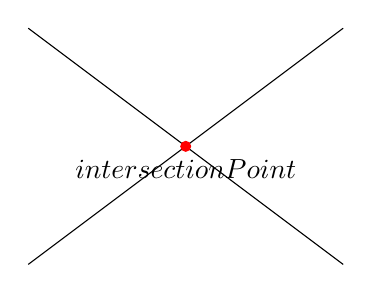
\begin{tikzpicture}
    \draw[name path=line1] (0, 0) -- (4, 3);
    \draw[name path=line2] (4, 0) -- (0, 3);

    \path[name intersections={of=line1 and line2, by={intersectionPoint}}];

    \fill[red] (intersectionPoint) circle (2pt);
    \node [fill=red,inner sep=1pt,label=-90:$intersectionPoint$] at (intersectionPoint) {};

    % \node at (intersectionPoint) {Intersection};
\end{tikzpicture}

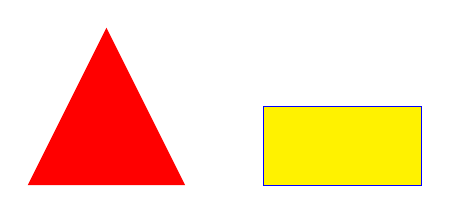
\begin{tikzpicture}
    \fill[red] (0, 0) -- (2, 0) -- (1, 2) -- cycle;
    \filldraw[blue, fill=yellow] (3, 0) rectangle (5, 1);
\end{tikzpicture}

\begin{tikzpicture}
    % Draw the rectangle
    \draw (0,0) rectangle (3,2);

    % Add characters at each corner
    \node[anchor=south east] at (0,0) {A}; % Bottom-left
    \node[anchor=south west] at (3,0) {B}; % Bottom-right
    \node[anchor=north west] at (3,2) {C}; % Top-right
    \node[anchor=north east] at (0,2) {D}; % Top-left
\end{tikzpicture}


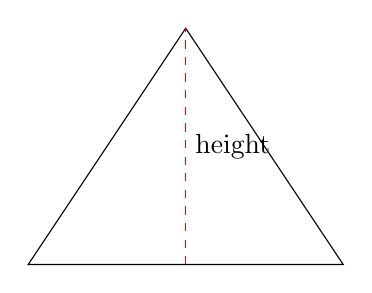
\begin{tikzpicture}
    \def\base{4}      % Length of the base
    \def\height{3}    % Height of the triangle
    \def\halfbase{\base/2} % Half of the base

    % Draw the triangle
    \draw (0,0) -- (\base,0) -- (\halfbase,\height) -- cycle;

    % Draw the height (optional)
    \draw[dashed, red] (\halfbase,0) -- (\halfbase,\height);

    % Label the height (optional)
    \node[right] at (\halfbase,\height/2) {height};
\end{tikzpicture}

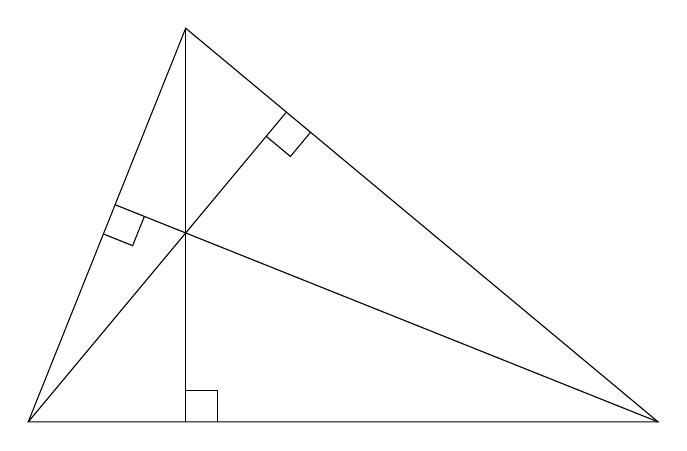
\begin{tikzpicture}[scale=2]
    \coordinate (A) at (0,0);
    \coordinate (B) at (1,2.5);
    \coordinate (C) at (4,0);
    \draw (A) -- (B) -- (C) -- cycle;
    \draw (B) -- ($(A)!(B)!(C)$) ++(90:0.2) -- ++(0:0.2) -- +(-90:0.2);
    \draw (A) -- ($(B)!(A)!(C)$) ++(-39.806:0.2) -- ++(50.194:-0.2) -- +(-39.806:-0.2);
    \draw (C) -- ($(A)!(C)!(B)$) ++(68.2:-0.2) -- ++(-21.8:0.2) -- +(68.2:0.2);
\end{tikzpicture}









\end{document}